\section{Injections}
\label{sec:intro_injections}

In this chapter you will learn how to implement methods that you cannot express as SDMs by adding handwritten code to classes created from your model.

Injections are inspired by the partial classes in C\#, our preferred way of doing this and a clean separation of generated from handwritten code.

\begin{enumerate}
    \item[$\blacktriangleright$] In order to implement \texttt{Box::addToStringRep} right-click on your class \texttt{Box} in Eclipse and choose ``eMoflon$\rightarrow$Create injection for class'' (Fig.~\ref{fig:injection_create_injection}).

    \begin{figure}[htbp]
        \centering
        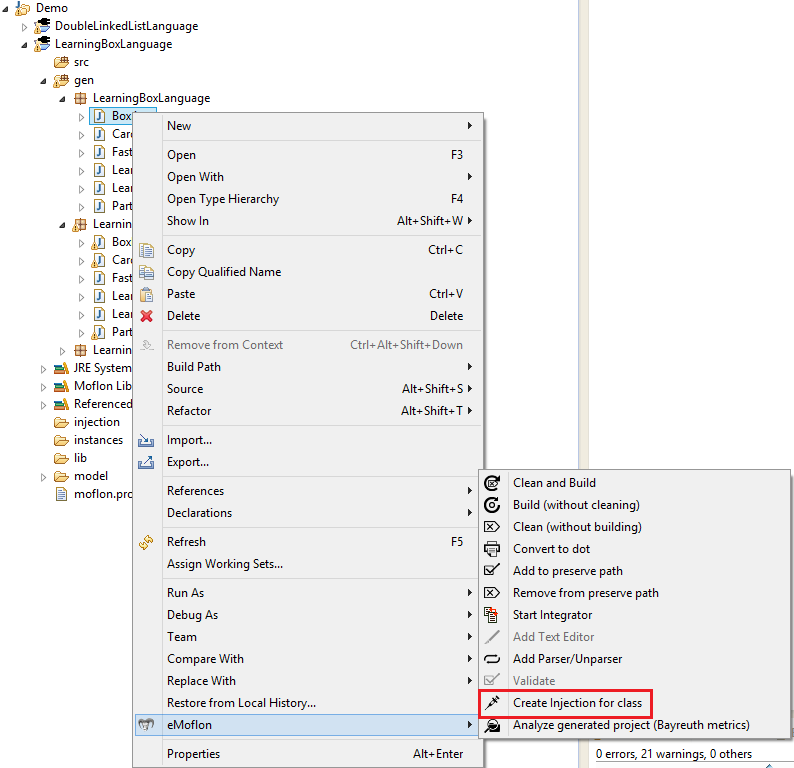
\includegraphics[width=\textwidth]{pics/injectionBilder/create_injection_context_menu.png}
        \caption{Create a new injection}
        \label{fig:injection_create_injection}
    \end{figure}

    This creates a new file in the \texttt{injection} folder of your project with the same packages and name as the Java class but with ``.inject'' as extension (Fig. \ref{fig:injection_created_injection_file}). This file contains the definition of a \textit{partial class} (Fig. \ref{code:empty_inject_file}). 

    \begin{figure}[htbp]
        \centering
        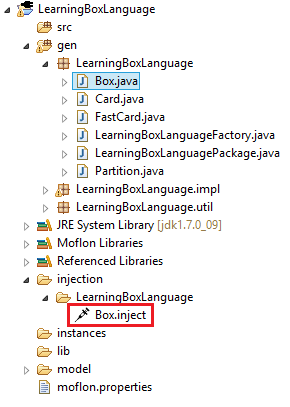
\includegraphics[width=0.6\textwidth]{pics/injectionBilder/newly_created_injection_file.png}
        \caption{Create a new injection}
        \label{fig:injection_created_injection_file}
    \end{figure}
    \FloatBarrier

    \lstdefinelanguage{Injection}[]{Java}{
        morekeywords={partial, class},
        sensitive=false,
        keywordstyle={\bfseries\color{purple}},
        emph={@model},
        emphstyle={\color{blue}},
        backgroundcolor=\color{white}
    }

    \begin{figure}[htbp]
        \centering
        \begin{lstlisting}[language=Injection]
            partial class Box
            {

            }
        \end{lstlisting}
        \caption{Empty injection file}
        \label{code:empty_inject_file}
    \end{figure}
    \FloatBarrier

    \item[$\blacktriangleright$]Now copy and paste the code in Fig. \ref{code:complete_inject_file} into your injection file.

    \begin{figure}[htbp]
        \centering
        \begin{lstlisting}[language=Injection]
            partial class Box
            {
                @model addToStringRep(Card card) <--
                    StringBuilder sb = new StringBuilder();
                    if (stringRep == null)
                    {
                        sb.append("BoxContent: [");
                    }
                    else
                    {
                        sb.append(stringRep);
                        sb.append(", [");
                    }
                    sb.append(card.getFace());
                    sb.append(", ");
                    sb.append(card.getBack());
                    sb.append("]");
                    stringRep = sb.toString();
                -->
            }
        \end{lstlisting}
        \caption{Implementation of helper method as an injection}
        \label{code:complete_inject_file}
    \end{figure}
    \FloatBarrier
    \item[$\blacktriangleright$] Rebuild your project (eMoflon $\rightarrow$ Clean and build) and this code will be injected in \texttt{LearningBoxLanguage.impl.BoxImpl.java} (Fig. \ref{fig:injected_code_in_boxImpl}). For more information on injections, read \ref{sec:appendix_injections}.

\end{enumerate}

    

    \begin{figure}[htbp]
        \centering
        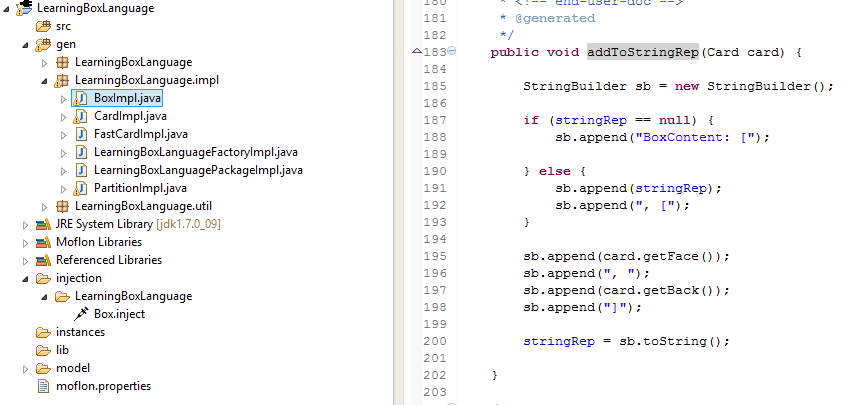
\includegraphics[width=\textwidth]{pics/injectionBilder/injected_code_in_impl.png}
        \caption{Injected code in BoxImpl after code generation}
        \label{fig:injected_code_in_boxImpl}
    \end{figure}